L'objectif de ce TP est de pouvoir transformer un modèle en texte à l'aide de l'outil Acceleo.

\section{Transformation de modèle à texte avec Acceleo}

Dans un premier temps on s'intéresse aux transformations à partir de modèle simplePDL.
Ces modèles sont exportés dans des fichiers textes respectant la syntaxe PDL1 et la syntaxe DOT.\\

Voilà par exemple le template pour la syntaxe PDL1 :\\

\lstset{language={}}
\begin{lstlisting}[caption=toPDL1.mtl]
[comment encoding = UTF-8 /]
[module toPDL1('http://simplepdl')]

[comment Generation de la syntaxe PDL1 à partir d'un modèle de processus /]

[template public toPDL(proc : Process)]
[comment @main/]
[file (proc.name.concat('.pdl1'), false, 'UTF-8')]
process [proc.name/]{
[for (wd : WorkDefinition | proc.processElements->getWDs())]
   wd [wd.name/]
[/for]
[for (ws : WorkSequence | proc.processElements->getWSs())]
   ws [ws.predecessor.name/] [ws.getWSType()/] [ws.successor.name/]
[/for]
}
[/file]
[/template]

[query public getWDs(elements : OrderedSet(ProcessElement)) : OrderedSet(WorkDefinition) = 
   elements->select( e | e.oclIsTypeOf(WorkDefinition) )
      ->collect( e | e.oclAsType(WorkDefinition) )
      ->asOrderedSet()
/]

[query public getWSs(elements : OrderedSet(ProcessElement)) : OrderedSet(WorkSequence) = 
   elements->select( e | e.oclIsTypeOf(WorkSequence) )
      ->collect( e | e.oclAsType(WorkSequence) )
      ->asOrderedSet()
/]

[template public getWSType(ws : WorkSequence)]
[if (ws.linkType = WorkSequenceType::startToStart)]
s2s[elseif (ws.linkType = WorkSequenceType::startToFinish)]
s2f[elseif (ws.linkType = WorkSequenceType::finishToStart)]
f2s[elseif (ws.linkType = WorkSequenceType::finishToFinish)]
f2f[/if]
[/template]

\end{lstlisting}

Les principales structures que l'on remarque sont les "template" qui permettent de mettre en page dynamiquement des bouts de code avec les objets transmis en paramètre et les "query" qui permettent de récupérer des ensembles sur lesquels on pourra itérer.\\

En s'inspirant de ce modèle, j'ai fait un template pour la transformation vers fichier ".dot".

\begin{lstlisting}[caption=toDot.mtl]
[comment encoding = UTF-8 /]
[module toDot('http://simplepdl')]

[comment Generation de la syntaxe dot à partir d'un modèle de processus /]

[template public toDot(proc : Process)]
[comment @main/]
[file (proc.name.concat('.dot'), false, 'UTF-8')]
digraph [proc.name/]{
[for (ws : WorkSequence | proc.processElements->getWSs())]
	[ws.predecessor.name/]->[ws.successor.name/]
[/for]
}
[/file]
[/template]

[query public getWSs(elements : OrderedSet(ProcessElement)) : OrderedSet(WorkSequence) = 
	elements->select( e | e.oclIsTypeOf(WorkSequence) )
		->collect( e | e.oclAsType(WorkSequence) )
		->asOrderedSet()
/]
\end{lstlisting}

Avec ce template on peut transformer le modèle de processus suivant en format texte :

\begin{center}
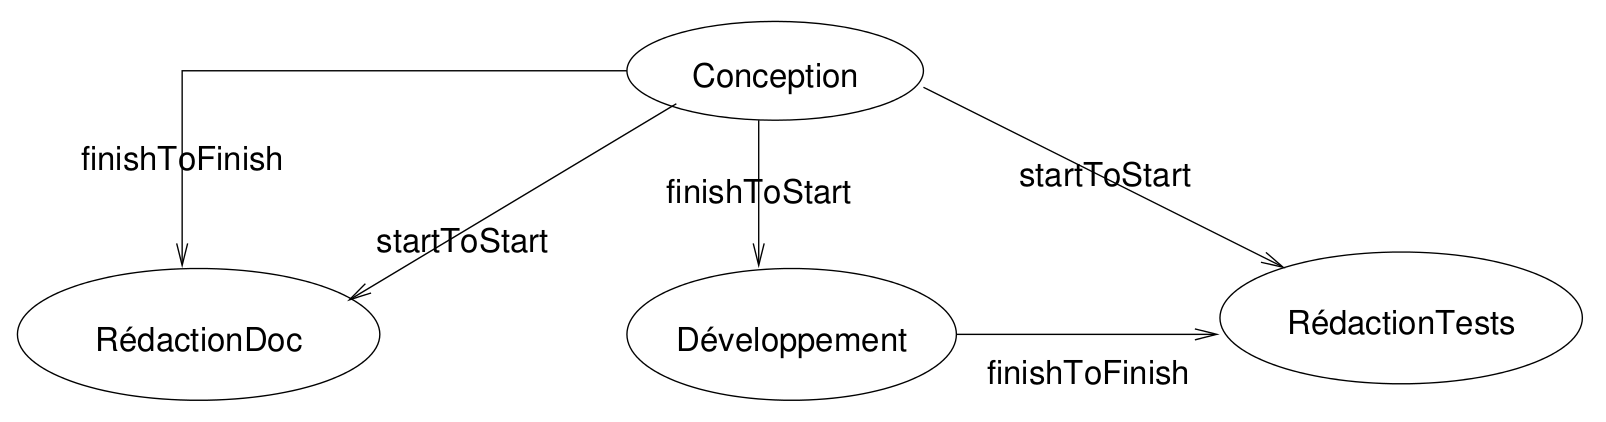
\includegraphics[width = 0.5\textwidth]{../Images/tp2/tp2_2-1.png}
\end{center}

et on obtient :

\begin{lstlisting}[caption=process.dot]
digraph process{
	Conception->RedactionDoc
	Conception->RedactionDoc
	Conception->Developpement
	Conception->RedactionTests
	Developpement->RedactionTests
}
\end{lstlisting}

\section{Application aux réseaux de Petri}

On transforme maintenant des modèles de réseau de pétri en texte. On fera un template pour fichier".net" et un template pour fichier ".dot". Le modèle de réseau de pétri nous servant d'example sera le même que celui du sujet, à savoir :

\begin{center}
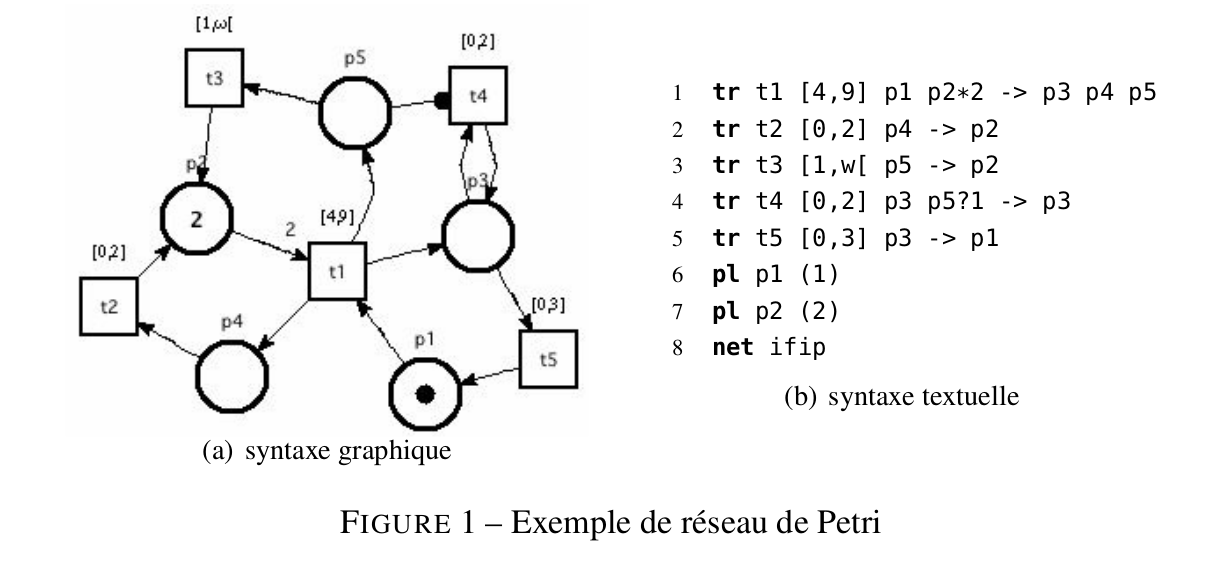
\includegraphics[width = 0.9\textwidth]{../Images/tp4/tp4_1.png}
\end{center}

On obtient les fichiers texte suivants :

\begin{lstlisting}[caption=example.net]
tr t1 p1 p2*2 -> p3 p4 p5
tr t2 p4 -> p2
tr t3 p5 -> p2
tr t4 p3 p5?1 -> p3
tr t5 p3 -> p1
pl p1 (1)
pl p2 (2)
net example
\end{lstlisting}

\begin{lstlisting}[caption=example.dot]
digraph example {
	t1 [shape=box];
	t2 [shape=box];
	t3 [shape=box];
	t4 [shape=box];
	t5 [shape=box];

	p1 [label="1"]
	p2 [label="2"]
	p3 [label=" "]
	p4 [label=" "]
	p5 [label=" "]

	p1 -> t1;
	p2 -> t1 [label="2"] ;
	p3 -> t4;
	p3 -> t5;
	p4 -> t2;
	p5 -> t3;
	p5 -> t4;
	t1 -> p3;
	t1 -> p4;
	t1 -> p5;
	t2 -> p2;
	t3 -> p2;
	t4 -> p3;
	t5 -> p1;
}
\end{lstlisting}

Le fichier example.dot une fois affiché donne ceci :

\begin{center}
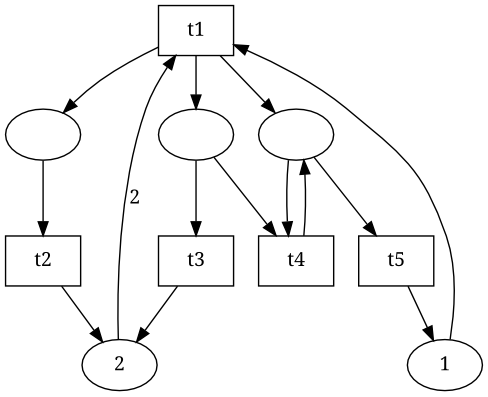
\includegraphics[width = 0.5\textwidth]{../Images/tp4/example.png}
\end{center}

On remarque que certaines améliorations sont possibles. On pourrait par example changer la couleur d'un read-arc et ajouter le nom d'une place en plus de son marquage dans les places.

Les codes des templates sont les suivants :

\begin{lstlisting}[caption=toNet.mtl]
[comment encoding = UTF-8 /]
[module toNet('http://petrinet/1.0')]

[comment Generation de la syntaxe .net à partir d'un modèle de réseau de pétri /]

[template public toNet(petriNet : PetriNet)]
[comment @main/]
[file (petriNet.name.concat('.net'), false, 'UTF-8')]
[for (tr : Transition | petriNet.petriNetElements->getTransitions())]
tr [tr.name/][tr.getTransitionsPredecessors()/] ->[tr.getTransitionsSuccessors()/]
[/for]
[for (pl : Place | petriNet.petriNetElements->getPlaces())]
[if (pl.marking > 0)]pl [pl.name/] ([pl.marking/])[/if]
[/for]
net [petriNet.name/]
[/file]
[/template]

[query public getTransitions(elements : OrderedSet(PetriNetElement)) : OrderedSet(Transition) = 
	elements->select( e | e.oclIsTypeOf(Transition) )
		->collect( e | e.oclAsType(Transition) )
		->asOrderedSet()
/]

[query public getPlaces(elements : OrderedSet(PetriNetElement)) : OrderedSet(Place) = 
	elements->select( e | e.oclIsTypeOf(Place) )
		->collect( e | e.oclAsType(Place) )
		->select( e | e.marking > 0 )
		->asOrderedSet()
/]

[template public getTransitionsPredecessors(tr : Transition)]
[for (arc : Arc | tr.linksToPredecessor)] [arc.getPredecessorPlace()/][/for]
[/template]

[template public getTransitionsSuccessors(tr : Transition)]
[for (arc : Arc | tr.linksToSuccessor)] [arc.getSuccessorPlace()/][/for]
[/template]

[template public getPredecessorPlace(arc : Arc)]
[arc.predecessor.name/][if (arc.readOnly)]?[arc.multiplicity/][elseif (arc.multiplicity > 1)]*[arc.multiplicity/][/if]
[/template]

[template public getSuccessorPlace(arc : Arc)]
[arc.successor.name/][if (arc.multiplicity > 1)]*[arc.multiplicity/][/if]
[/template]
\end{lstlisting}

\begin{lstlisting}[caption=toDot.mtl]
[comment encoding = UTF-8 /]
[module toDot('http://petrinet/1.0')/]

[comment Generation de la syntaxe .dot à partir d'un modèle de réseau de pétri /]

[template public toDot(petriNet : PetriNet)]
[comment @main/]
[file (petriNet.name.concat('.dot'), false, 'UTF-8')]
digraph [petriNet.name/] {
	[for (tr : Transition | petriNet.petriNetElements->getTransitions())]
	[tr.name/] ['box'.getShape()/];
	[/for]

	[for (pl : Place | petriNet.petriNetElements->getPlaces())]
	[pl.name/] [if (pl.marking > 0)][pl.marking.toString().getLabel()/][else][' '.getLabel()/][/if]
	[/for]

	[for (arc : Arc | petriNet.petriNetElements->getArcs())]
	[arc.predecessor.name/] -> [arc.successor.name/][if (arc.multiplicity > 1)] [arc.multiplicity.toString().getLabel()/] [/if];
	[/for]
}
[/file]
[/template]

[query public getTransitions(elements : OrderedSet(PetriNetElement)) : OrderedSet(Transition) = 
	elements->select( e | e.oclIsTypeOf(Transition) )
		->collect( e | e.oclAsType(Transition) )
		->asOrderedSet()
/]

[query public getPlaces(elements : OrderedSet(PetriNetElement)) : OrderedSet(Place) = 
	elements->select( e | e.oclIsTypeOf(Place) )
		->collect( e | e.oclAsType(Place) )
		->asOrderedSet()
/]

[query public getArcs(elements : OrderedSet(PetriNetElement)) : OrderedSet(Arc) = 
	elements->select( e | e.oclIsTypeOf(Arc) )
		->collect( e | e.oclAsType(Arc) )
		->asOrderedSet()
/]

[template public getLabel(s : String)]
['['/]label="[s/]"[']'/]
[/template]

[template public getShape(s : String)]
['['/]shape=[s/][']'/]
[/template]
\end{lstlisting}

